\documentclass[main.tex]{subfiles}
\begin{document}\newpage
\setdoublesep{0.35700 em}  % 'Bond Spacing'
\setatomsep{1.78500 em}    % 'Fixed Length'
\setbondoffset{0.18265 em} % 'Margin Width'
\newcommand{\bondwidth}{0.06642 em} % 'Line Width'
\setbondstyle{line width = \bondwidth}
\taburulecolor{black}


 


%%%%%%%%%%%%HEADING
\begin{multicols}{2}
\begin{tcolorbox}[enhanced jigsaw,breakable,size=title,
colback=mybrown!05,colframe=black,fonttitle=\bfseries,
title=STUDENT INFO,pad at break=1mm, break at=15cm/0pt ]
\vspace{0.2cm}
\noindent Name: \rule{5cm}{0.4pt}Date:\rule{1cm}{0.4pt}\\
\end{tcolorbox}
\end{multicols}
\hfill
\vspace{0.2cm}
\begin{center}
{\large \bfseries 
Pre-lab Questions 
\par
\Huge
Chemistry and measurements
\\[5pt] \par}
\vspace{0.2cm}
\end{center}
\par
\noindent
\uline{  \hfill \normalsize \hfill       }
%%%%%%%%%%%%HEADING

\begin{enumerate}
% PELAB 1
\item Fill the gaps with the full unit name, the abbreviation and the property measured. Indicate also whether the unit contains a prefix:
\vspace{1cm}
\begin{center}
 \begin{tabular}{ p{3cm} p{3cm} p{3cm}p{3cm}   }
   \begin{bf}Full unit Name\end{bf} & \begin{bf}Abbreviation\end{bf} &\begin{bf}Property measured\end{bf} &\begin{bf}Prefix? (yes/no)\end{bf} \\[0.1cm]     
  Kilogram 				&\rule{3cm}{0.4pt}&\rule{3cm}{0.4pt}&\rule{3cm}{0.4pt}  \\[0.1cm]      
    \rule{3cm}{0.4pt}&mL& \rule{3cm}{0.4pt}&\rule{3cm}{0.4pt}       \\[0.1cm]
     Degree Celsius 				&\rule{3cm}{0.4pt}&\rule{3cm}{0.4pt}&\rule{3cm}{0.4pt}  \\[0.1cm]      
    \rule{3cm}{0.4pt}&in& \rule{3cm}{0.4pt}&\rule{3cm}{0.4pt}       \\[0.1cm]
 \end{tabular}
 \end{center}
\vspace{.5cm}





\item Indicate whether the following numbers indicate a measured value or an exact number. Measured numbers result from measurements, and  exact numbers result from counting.\\
\vspace{1cm}
 \begin{tabular}{ p{3cm} p{3cm} p{3cm}p{3cm}   }
  20Kg 				&\rule{3cm}{0.4pt}&10.5 cm&\rule{3cm}{0.4pt}  \\[0.1cm]      
    3 apples 				&\rule{3cm}{0.4pt}&10$^{\circ}$C&\rule{3cm}{0.4pt}  \\[0.1cm]      
  30.5L				&\rule{3cm}{0.4pt}&90mL&\rule{3cm}{0.4pt}  \\[0.1cm]      
  1cm=$10^{-2}$m				&\rule{3cm}{0.4pt}&4g&\rule{3cm}{0.4pt}  \\[0.1cm]      

 \end{tabular}
\vspace{.5cm}

\item Explain what are significant figures.
\vspace{2cm}


\item You measure the mass of a beaker using a scale and the results is 28.27g. Indicate the estimated digit of the measurement.
\vspace{1cm}


\item You measure the length of a measuring cylinder using a meter stick with a scale that indicates centimeter as well as millimeters and the results is 25.15cm. Indicate the estimated digit of the measurement.
\vspace{3cm}



\end{enumerate}


\clearpage\mbox{}\clearpage



%%%%%%%%%%%%HEADING
\begin{multicols}{2}
\begin{tcolorbox}[enhanced jigsaw,breakable,size=title,
colback=mybrown!05,colframe=black,fonttitle=\bfseries,
title=STUDENT INFO,pad at break=1mm, break at=15cm/0pt ]
\vspace{0.2cm}
\noindent Name: \rule{5cm}{0.4pt}Date:\rule{1cm}{0.4pt}\\
\end{tcolorbox}
\end{multicols}
\hfill
\vspace{0.2cm}
\begin{center}
{\large \bfseries 
Experiment
\par
\Huge
Chemistry and measurements
\\[5pt] \par}
\vspace{0.2cm}
\end{center}
\par
\noindent
\uline{  \hfill \normalsize \hfill       }
%%%%%%%%%%%%HEADING

\vspace{0.2cm}{\large \bfseries 1. Measuring mass}
The goal of this mini-experiment is to measure the mass of several objects with a scale. Overall, the goal is to learn how to use laboratory scales and how to properly report measurements. Moreover, this experiment will help you getting familiarized with a chemistry laboratory environment:

\begin{steps}
    \newstep[] Locate the following objects: a 10ml measuring cylinder, a 50ml beaker, a stopper of any size and a spatula.     
    \newstep[] Measure the mass of each of the object using a scale. Make sure the scale is set to zero before you measure. 
    \newstep[]Write down the values listing the name of the object. Do not forget to indicate the unit of the measurement.
    \newstep[] Indicate the measured figure (e.g. for a measure number 345.8g the estimated would be written as 0.8g) and the number of significant figures of the measurement.
     \newstep[] Return each object to its original location in the lab.
\end{steps}

\begin{center} \begin{tabular}{ p{5cm} p{3cm} p{3cm}p{3cm}   }
   \begin{bf}Object Name\end{bf} & \begin{bf}Mass\end{bf} &\begin{bf}Estimated digit\end{bf} &\begin{bf}\# significant Figures\end{bf} \\[0.1cm]     
  \rule{5cm}{0.4pt} 				&\rule{3cm}{0.4pt}&\rule{3cm}{0.4pt}&\rule{3cm}{0.4pt}  \\[0.2cm]      
  \rule{5cm}{0.4pt} 				&\rule{3cm}{0.4pt}&\rule{3cm}{0.4pt}&\rule{3cm}{0.4pt}  \\[0.2cm]      
  \rule{5cm}{0.4pt} 				&\rule{3cm}{0.4pt}&\rule{3cm}{0.4pt}&\rule{3cm}{0.4pt}  \\[0.2cm]      
  \rule{5cm}{0.4pt} 				&\rule{3cm}{0.4pt}&\rule{3cm}{0.4pt}&\rule{3cm}{0.4pt}  \\[0.2cm]      
 \end{tabular}\end{center}


\vspace{0.2cm}{\large \bfseries 2. Measuring length}
In this mini-experiment you will familiarize with a meterstick (or a inch ruler). I am aware you have seen one before but perhaps you have not noticed some of the nuances of this very useful measuring tool.Think about the meaning of the large and small lines on the meterstick (or a inch ruler). Discuss with your coworkers this information. What do the large lines represent? And the small lines?

\begin{steps}
    \newstep[] Write down the length of the following items. Mind you need to measure these values in the lab. In the case of your height, you will find a meter stick at the lab, near the entrance. 
      \newstep[] You can use a string to measure the length of your wrist .
     \newstep[] Write down the measured digit of each measurement and the number of significant figures. Do not forget to indicate the unit near the measurement.

 
\begin{center} \begin{tabular}{ p{5cm} p{3cm} p{3cm}p{3cm}   }
   \begin{bf}Object Name\end{bf} & \begin{bf}Length\end{bf} &\begin{bf}Estimated digit\end{bf} &\begin{bf}\# SFs\end{bf} \\[0.1cm]     
  Length of your right foot 				&\rule{3cm}{0.4pt}&\rule{3cm}{0.4pt}&\rule{1cm}{0.4pt}  \\[0.3cm]      
  Length of one of your fingernails 				&\rule{3cm}{0.4pt}&\rule{3cm}{0.4pt}&\rule{1cm}{0.4pt}  \\[0.3cm]      
  Length of one of your wrist 				&\rule{3cm}{0.4pt}&\rule{3cm}{0.4pt}&\rule{1cm}{0.4pt}  \\[0.3cm]   
    Line below 				&\rule{3cm}{0.4pt}&\rule{3cm}{0.4pt}&\rule{1cm}{0.4pt}  \\[0.3cm]      
 \end{tabular}
 \end{center}
 
  \newstep[] Measure the length of the following line and write down the value on the table above.
 \begin{center} \rule{7.5cm}{0.4pt}\end{center}
\end{steps}
 




 
 
\vspace{0.2cm}{\large \bfseries 3. Measuring volume}
In this mini-experiment learn how to properly read a volume measurement using chemistry equipment. In the chemistry lab, volume can be measured with a measuring cylinder. However, liquid forms a meniscus on this object due to a property of water called surface tension. Therefore, to be able to read volume you will have to properly read the meniscus and use volumetric scales.
\begin{steps}
    \newstep[] Locate the lab setup with measuring cylinders of 10, 25, 50, 100 and 250 mL.
        \newstep[]  Fill each cylinder with a random quantity if water within the volume of the cylinders. The cylinders might be already filled.
        \newstep[]  For each cylinder, read the meniscus and write down the volume. Make sure you read between the lines of the cylinder to indicate the estimated digit of the measurement. Do not forget to write down the unit close to the measurement.
         \newstep[] Indicate the estimated digit of the measurement and the number of significant figures.     
\end{steps}

\begin{center} \begin{tabular}{ p{5cm} p{3cm} p{3cm}p{3cm}   }
   \begin{bf}Object Name\end{bf} & \begin{bf}Volume\end{bf} &\begin{bf}Estimated digit\end{bf} &\begin{bf}\# SFs\end{bf} \\[0.1cm]     
  \rule{5cm}{0.4pt} 				&\rule{3cm}{0.4pt}&\rule{3cm}{0.4pt}&\rule{1cm}{0.4pt}  \\[0.3cm]      
  \rule{5cm}{0.4pt} 				&\rule{3cm}{0.4pt}&\rule{3cm}{0.4pt}&\rule{1cm}{0.4pt}  \\[0.3cm]      
  \rule{5cm}{0.4pt} 				&\rule{3cm}{0.4pt}&\rule{3cm}{0.4pt}&\rule{1cm}{0.4pt}  \\[0.3cm]      
  \rule{5cm}{0.4pt} 				&\rule{3cm}{0.4pt}&\rule{3cm}{0.4pt}&\rule{1cm}{0.4pt}  \\[0.3cm]      
  \rule{5cm}{0.4pt} 				&\rule{3cm}{0.4pt}&\rule{3cm}{0.4pt}&\rule{1cm}{0.4pt}  \\[0.3cm]      
 \end{tabular}\end{center}


\vspace{0.2cm}{\large \bfseries 5. Measuring volume by displacement }
The volume of liquids is easy to measure. However, the volume of solids is a harder property to measure experimentally. The goal of this mini-experiment is to measure the volume of an object (a cylindric piece of metal) by displacing the liquid on a measuring cylinder.
\begin{steps}
        \newstep[]  Find a metallic cylinder you want to measure volume.
    \newstep[] Use a 50mL-cylinder large enough to easily fit the object. Make sure the object will not be stuck inside the cylinder.      
    \newstep[] Add water to the cylinder and write down the volume. Make sure you read the estimated digits (e.g. 50.50mL).
            \newstep[] Place the object on the cylinder. You will see the level of water rise. Make sure the level is beyond the size of the object so that the object is fully submerged on water. If not, you will have to repeat the experiment adding more water initially on the cylinder.
               \newstep[] Calculate the volume of the object by subtracting the the volume of water after the object is submerged--the final volume--and the volume before--the initial volume.
   \end{steps}
\begin{center} \begin{tabular}{ p{3cm} p{3cm}p{3cm} p{3cm}p{3cm}   }
  & &\begin{bf}Volume\end{bf} &\begin{bf}Estimated digit\end{bf} &\begin{bf}\# SFs\end{bf} \\[0.1cm]     

 \begin{bf}Initial volume\end{bf}		&\centering\mycircled{1}		&\rule{3cm}{0.4pt}&\rule{3cm}{0.4pt}&\rule{1cm}{0.4pt}  \\[0.3cm]      
 \begin{bf}Final volume\end{bf}		&\centering\mycircled{2}		&\rule{3cm}{0.4pt}&\rule{3cm}{0.4pt}&\rule{1cm}{0.4pt}  \\[0.3cm]      
 \begin{bf}Object volume\end{bf} 	&\centering\mycircled{2} \, - \, \mycircled{1}				&\rule{3cm}{0.4pt}&\rule{3cm}{0.4pt}&\rule{1cm}{0.4pt}  \\[0.3cm]      
 \end{tabular}\end{center}


 
\clearpage\mbox{}\clearpage


\newpage
 

%%%%%%%%%%%%HEADING
\begin{multicols}{2}
\begin{tcolorbox}[enhanced jigsaw,breakable,size=title,
colback=mybrown!05,colframe=black,fonttitle=\bfseries,
title=STUDENT INFO,pad at break=1mm, break at=15cm/0pt ]
\vspace{0.2cm}
\noindent Name: \rule{5cm}{0.4pt}Date:\rule{1cm}{0.4pt}\\
\end{tcolorbox}
\end{multicols}
\hfill
\vspace{0.2cm}
\begin{center}
{\large \bfseries 
Post lab
\par
\Huge
Chemistry and measurements
\\[5pt] \par}
\vspace{0.2cm}
\end{center}
\par
\noindent
\uline{  \hfill \normalsize \hfill       }
%%%%%%%%%%%%HEADING




\begin{enumerate}
\item 
   Indicate the measurement of the following meniscus (in mL):
\begin{figure*}[h] % FUL FIGURE
        %  \includegraphics[width=\textwidth]{../Ch-measurements/LAB-GOB-Chemistryandmeasurements/measure2.png}
          \includegraphics[width=\textwidth]{measure2.png}
\end{figure*}
%\begin{center} \begin{tabular}{ p{3cm}p{3cm} p{3cm}p{3cm}   }
%\hspace{0.1cm}\rule{2cm}{0.4pt}	&\hspace{0.1cm}\rule{2cm}{0.4pt}&\hspace{0.1cm}\rule{2cm}{0.4pt}&\hspace{0.1cm}\rule{2cm}{0.4pt}  \\     
% \end{tabular}\end{center}
%
%\hspace{1cm}\rule{2cm}{0.4pt}	 \hspace{0.1cm}\rule{2cm}{0.4pt} \hspace{0.1cm}\rule{2cm}{0.4pt} \hspace{0.1cm}\rule{2cm}{0.4pt}      


\vspace{1.5cm}
\item Using the rule below in cm:\\

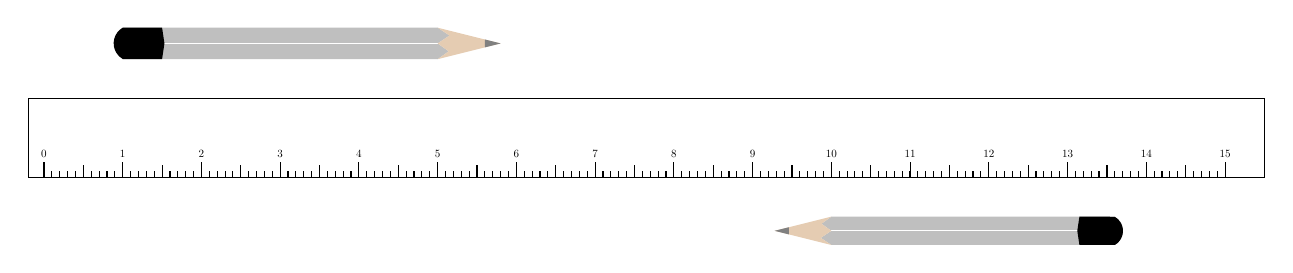
\begin{tikzpicture} 
\begin{scope}
            \draw (-0.2,0) rectangle (15.5,1);
            %% lower divisions
            \foreach \x in {0,1,...,15}{
            \draw (\x,0) -- (\x,0.2)node[above,scale=0.4]{\x};
            }
            \foreach \x in {0.1,0.2,...,14.9}{
            \draw (\x,0) -- (\x,0.075);
            }
            \foreach \x in {0.5,1,...,14.5}{
            \draw (\x,0) -- (\x,0.15);
            }
%            % Upper divisions
%            \foreach \x in {0,1,...,6}{
%            \draw (\x in,1) -- (\x in,0.8)node[below,scale=0.4]{\x};
%            }
%            \foreach \x in {0.1,0.2,...,5.9}{
%            \draw (\x in,1) -- (\x in,0.925);
%            }
%            \foreach \x in {0.5,1,...,5.5}{
%            \draw (\x in,1) -- (\x in,0.85);
%            }
\end{scope}

\begin{scope}[shift={(5,1.5)},rotate=90]
\fill[gray!50] (0,4) -- (0.4,4) -- (0.4,0) --(0.3,-0.15) -- (0.2,0) -- (0.1,-0.14) -- (0,0) -- cycle;
            \draw[color=white] (0.2,4) -- (0.2,0);
            \fill[black] (0,3.5) -- (0.2,3.47) -- (0.4,3.5) -- (0.4,4) arc(30:150:0.23cm);
            \fill[brown!40] (0,0) -- (0.2,-0.8)node[coordinate,pos=0.75](a){} -- (0.4,0)node[coordinate,pos=0.25](b){} -- (0.3,-0.15) -- (0.2,0) -- (0.1,-0.14) -- cycle;
            \fill[gray] (a) -- (0.2,-0.8) -- (b) -- cycle;   
            \end{scope}
\begin{scope}[shift={(10,-0.5)},rotate=-90, scale=0.9]
\fill[gray!50] (0,4) -- (0.4,4) -- (0.4,0) --(0.3,-0.15) -- (0.2,0) -- (0.1,-0.14) -- (0,0) -- cycle;
            \draw[color=white] (0.2,4) -- (0.2,0);
            \fill[black] (0,3.5) -- (0.2,3.47) -- (0.4,3.5) -- (0.4,4) arc(30:150:0.23cm);
            \fill[brown!40] (0,0) -- (0.2,-0.8)node[coordinate,pos=0.75](a){} -- (0.4,0)node[coordinate,pos=0.25](b){} -- (0.3,-0.15) -- (0.2,0) -- (0.1,-0.14) -- cycle;
            \fill[gray] (a) -- (0.2,-0.8) -- (b) -- cycle;   
            \end{scope}

                 \end{tikzpicture}

\begin{enumerate}
\item Measure the length of both pencils.
\vspace{1cm}
\item Indicate the estimated digits

\end{enumerate}
\vspace{1.5cm}

\item Indicate the number of significant figures of the following measurements:\\
\vspace{2cm}
 \begin{tabular}{ p{3cm} p{3cm} p{3cm}p{3cm}   }
   \begin{bf} Measured number\end{bf}		&   \begin{bf} SFs\end{bf}&\begin{bf} Measured number\end{bf}&\begin{bf} SFs\end{bf}  \\[0.1cm]      

  20.1Kg 				&\rule{3cm}{0.4pt}&			120.5 cm&\rule{3cm}{0.4pt}  \\[0.1cm]      
  0.01 m 				&\rule{3cm}{0.4pt}&			100g&\rule{3cm}{0.4pt}  \\[0.1cm]      
  0.010 s 				&\rule{3cm}{0.4pt}&			230.1dm&\rule{3cm}{0.4pt}  \\[0.1cm]      
  5$\times 10^{-5}$ dm 				&\rule{3cm}{0.4pt}&			6.500$\times 10^{-1}$ dmg&\rule{3cm}{0.4pt}  \\[0.1cm]      

 \end{tabular}

\vspace{2.5cm}

\end{enumerate}



 



\end{document}
